%--------------------------------------------------------%
%	BODY TEXT
%--------------------------------------------------------%

% Start double spacing
\doublespacing

% Main Text
\section{Introduction}

Mon stage d'étude en licence s'est déroulé au sein de l’UMR BIOGECO (Biodiversité Gènes \& Communautés) situé dans la station forestière INRAE de Cestas-Pierroton. Cette unité regroupe des agents de l'université de Bordeaux et du département ECODIV (Écologie et Biodiversité) de l’INRAE. L’activité de ce site est centrée autour de l’étude de la biodiversité et l'évolution des écosystèmes terrestres. Mon maître de stage, Cyril Dutech, y est chargé de recherche dans l’équipe GEMFOR (Génétique et écologie des maladies des forêts). Il s’intéresse à la diversité et à l'évolution des agents pathogènes des arbres forestiers.

Dans le cadre de mon stage, nous nous intéresserons au genre Armillaria\hyperref[bib:biblioI]{\textsuperscript{i}}.  Ce genre appartient à l'embranchement des Basidiomycètes de la famille des Physalacriaceae. Ces champignons se développent dans du bois aussi bien vivant (parasites) que mort (saprotrophes). Ils entraînent chez les arbres vivants une maladie, le pourridié-agaric\hyperref[bib:biblioII]{\textsuperscript{ii}}. Ils ont un impact notable sur la santé des forêts \cite{Shaw1991}. Ils participent certes à la dégradation du bois mort mais ont bien souvent des conséquences plus néfaste sur la santé des forêt, notamment des forêt âgées ou des plantations. Par ailleurs leur évolution face aux changements globaux et notamment face au réchauffement climatique \cite{Labbe2017} pourrait se révéler d'autant plus néfaste. Ils peuvent aussi présenter une menace en sylviculture, empêchant l'utilisation en bois d'\oe uvre et attaquant le bois stocké. Si il existe de nombreuses espèces d'Armillaire, notamment sur le continent nord-américain, nous étudierons plus particulièrement les espèces présentes en Europe\hyperref[bib:biblioIII]{\textsuperscript{iii}}.

L'identification des espèces d'Armillaire est une tâche délicate. Il existe plusieurs critères (morphologique, biologique, phylogénétique) qui présentent chacun certains avantages et certains inconvénients. Les Armillaires se reproduisent par reproduction sexuée, on peut donc se baser sur une identification morphologique de leur sporophore\hyperref[bib:biblioIV]{\textsuperscript{iv}} mais l'on peut aussi utiliser les thalles\hyperref[bib:biblioV]{\textsuperscript{v}} ou les rhizomorphes\hyperref[bib:biblioVI]{\textsuperscript{vi}}. Cependant trouver un sporophore n'est pas simple car cette reproduction n'intervenant qu'en fin d'automne, ces fructifications ne sont pas toujours disponibles. Pour ce qui est du critère biologique de l'espèce (la capacité de deux individus à se croiser et à donner des descendants viables et fertiles) il n'est pas toujours simple à utiliser car les barrières reproductives ne sont pas toujours strictes chez les Armillaires. Du plus, les spéciations allopatriques qui ont pu survenir mènent souvent à des isolements reproductifs incomplets. Enfin ce critère n'est pas toujours simple à utiliser car il nécessite de réaliser des isolements puis de tester cette barrière avec des souches référentes. Nous arrivons finalement au critère phylogénétique, basé sur la similarité de séquence nucléotidiques. Pour les champignons, la séquence dite marqueur universel est l'ITS\hyperref[bib:biblioVII]{\textsuperscript{vii}} \cite{Schoch2012, Chillali1998} mais il en existe aussi d'autres (RFLP, RAPD ou IGS). Ce critère est grandement utilisé, notamment avec le développement des outils d'analyse génétique et de séquençage. Elle présente elle aussi des limites. Lors de l'analyse d'un seul gène ou locus, il n'est parfois pas possible de séparer des espèces proches lorsqu'elles font parti d'un complexe d'espèces\hyperref[bib:biblioVIII]{\textsuperscript{viii}} (comme c'est le cas pour Armillaria) \cite{Taylor2000}. De plus, un polymorphisme intra-spécifique peut aussi compliquer cette distinction, limitant les variations fixées entres espèces. Contre ces travers, des méthodes prenant en compte plusieurs séquences ont été utilisées \cite{Tsykun2013}, rendant l'analyse plus fiable mais nécessitant plus de données génétiques, ce qui manque souvent. On utilise ici la congruence des phylogénies, lorsque les arbres de plusieurs gènes sont congruents cela démontre que le flux de gènes est interrompu depuis plusieurs générations, il n'y a ainsi plus de croisements viables ou possibles.

D'autres études se sont penchées sur ce dernier critère en se basant sur la séquence ITS  \cite{Kim2006, Coetzee2003}. Ainsi, chez les champignons, il est d'usage de séquencer l'ITS afin de construire des arbres phylogénétiques, mais deux limites apparaissent rapidement. Nous souhaiterions simplement identifier les espèces rapidement sur la base de leur variation nucléotidique et non construire des arbres qui reposent tout d'abord sur des hypothèses évolutives et des méthodes particulières (maximum de parcimonie ou maximum de vraisemblance \cite{Tamura2011, Sober2004}). En outre, ces méthodes nécessitent des séquences de bonne qualité avec assez d'information phylogénétique afin d'éviter des complications telles que l'attraction des longues branches \cite{Bergsten2005}. De plus l'ITS est parfois trop peu résolutif, notamment dans le cas de \textit{A. borealis} et \textit{A. ostoyae} \cite{Tsykun2013}. Une solution serait de voir si il n'existe pas des SNP\hyperref[bib:biblioIX]{\textsuperscript{ix}} diagnostiques entre espèces, c'est à dire différents entres espèces ou groupes d'espèces mais fixés au sein d'une même espèce ou groupe d'espèces \cite{Tsykun2017}. Quelques outils existent déjà, certain OpenSource comme SNPhood \cite{Arnold2016}, snpReady \cite{Granato2018} ou le très complet SeqQual \cite{Lang2021}. Cependant ce dernier à été programmé en Perl et Bash Unix, difficile donc d'approche pour moi. J'avais de plus la volonté de comprendre le fonctionnement et les rouages de ces outils. Ici, nous réinventerons donc en quelque sorte la roue en présentant une méthode complète de recherche automatique de SNPs et de détermination.

\section{Matériel et Méthodes}
% \setlength{\parindent}{0pt}

\textit{Isolats d'Armillaire} - Nous avons utilisé des isolats des six espèces du complexe des Armillaires. Ces isolats ont été récupérés à partir de rhizomorphes dans divers forêts françaises. Ces isolats ont été conservés par lyophilisation avant l'extraction d'ADN.

\textit{Extraction et séquençage de l'ADN} - L'ADN des isolats à été extrait par la méthode CTAB \cite{Gardes1993}. Les séquences ITS (ITS-1, 5.8S et ITS-2) de ces extractions d'ADN ont été amplifiées par PCR par des sondes spécifiques, et ensuite séquencées par la méthode de Sanger.

\textit{Détermination des SNPs} - Les SNPs diagnostiques de chaque espèce ont été obtenu par analyse de séquences de souches de référence\hyperref[ann:annexeA]{\textsuperscript{A}} identifiées par divers marqueurs génétiques \cite{Tsykun2013} mais dont certaines avaient été préalablement identifiées par des critères morphologiques et biologiques \cite{Guillaumin1991}.  D'autres séquences, identifiées par des critères morphologiques ou phylogénétiques, ont aussi été utilisées comme références\hyperref[ann:annexeA]{\textsuperscript{A}}. L'alignement de ces séquence\hyperref[ann:annexeB1] {\textsuperscript{B.1}} à été réalisé par l'algorithme MUSCLE 3.8.31 \cite{Edgar2004}. Ces séquences ont ensuite été nettoyées\hyperref[ann:annexeB2]{\textsuperscript{B.2}} en enlevant les sites contenant des gaps\hyperref[ann:annexeD1]{\textsuperscript{D.1}}, et cela pour plusieurs raisons. Premièrement, les commencements et fins de séquences contiennent souvent de nombreux

\singlespacing
\begin{tikzpicture}[node distance=2cm]

\node (start) [startstop] {\textit{Sequence Identifier Scripts}};
\node (in1a) [io, below of=start, xshift=-4cm, align=center] {Séquencces inconnues (.ab1)};
\draw [arrow] (start) -- (in1a);

    \node (pro1a) [process, below of=in1a, align=center] {ab1\_to\_fastQ.py\\ Filtre et compile les séquences selon leur phred scores.};
    \draw [arrow] (in1a) -- (pro1a);
    \node (out1a) [io, below of=pro1a] {*.fas};
    \draw [arrow] (pro1a) -- (out1a);

    \node (pro2a) [process, below of=out1a, align=center] {align\_ref\_unk.py\\ Réalise un alignement avec les séquences de référence.};
    \draw [arrow] (out1a) -- (pro2a);
    \node (out2a) [io, below of=pro2a] {*\_aligned.fasta};
    \draw [arrow] (pro2a) -- (out2a);

    \node (pro3a) [process, below of=out2a, align=center] {filter\_alignement.py\\ Enlève de l'alignement les indels.};
    \draw [arrow] (out2a) -- (pro3a);
    \node (out3a) [io, below of=pro3a] {*\_aligned\_cleaned.fasta};
    \draw [arrow] (pro3a) -- (out3a);

    \node (pro4a) [process, below of=out3a, align=center] {snp\_identifier.py\\ Identifie les séquences à partir du fichier de SNPs.};
    \draw [arrow] (out3a) -- (pro4a);
    \node (out4a) [io, below of=pro4a] {*\_species.JSON};
    \draw [arrow] (pro4a) -- (out4a);

\node (in1c) [io, below of=start, xshift=+4cm, align=center] {Liste d'espèces};
\draw [arrow] (start) -- (in1c);

    \node (pro1c) [process, below of=in1c, align=center] {GenBank\_scrap.py\\ Téléchargement de séquenques sur GenBank.};
    \draw [arrow] (in1c) -- (pro1c);
    \node (out1c) [io, below of=pro1c, align=center] {genbank\_A.fas};
    \draw [arrow] (pro1c) -- (out1c);
    \draw [arrow] (out1c) -- (pro2a);

\node (in1b) [io, below of=out1c, yshift=-2cm, align=center] {Séquencces reférentes (.fasta)};
\draw [arrow] (in1b) -- (pro2a);

    \node (pro1b) [process, below of=in1b, align=center] {consensus\_sequence.py\\ Détermine les sites polymorphes.};
    \draw [arrow] (in1b) -- (pro1b);
    \node (out1b) [io, below of=pro1b] {consensus\_seq.csv};
    \draw [arrow] (pro1b) -- (out1b);

    \node (pro2b) [process, below of=out1b, align=center] {snps.R\\ Détermine les SNPs diagnostiques.};
    \draw [arrow] (out1b) -- (pro2b);
    \node (out2b) [io, below of=pro2b, align=center] {snps.csv\\snps\_out\_group.csv};
    \draw [arrow] (pro2b) -- (out2b);
    \draw [arrow] (out2b) -- (pro4a);

\node[below of=out2b, xshift=1cm, yshift=1cm] {Figure 1 - Organigramme du script};

\end{tikzpicture}
\doublespacing

\noindent
gaps après alignement. Deuxièmement de trop nombreux gaps peuvent mener à des erreurs d'alignement, notamment lorsque que nous effectuerons celui entre séquences de référence et séquences inconnues. Enfin les gaps sont la marque d'insertions ou de délétions (indels) qui se trouvent être souvent des erreurs de séquençage. Ensuite, pour la validation d'un SNP\hyperref[ann:annexeD2]{\textsuperscript{D.2}}, nous avons fixé plusieurs règles:
\renewcommand{\labelitemi}{$\bullet$}
\begin{itemize}
    \item Pas de polymorphisme intraspécifique
    \item Le SNP doit être fixé
\end{itemize}

Nous avons, en sortie, des tableaux rassemblant les SNPs recensés et l'espèce à laquelle ils correspondent\hyperref[ann:annexeC2]{\textsuperscript{C}}.

\textit{Test sur séquences issue de NCBI} - La première mise en pratique de cette méthode se fera sur des séquences récupérées sur GenBank dont on connaît déjà l'espèce. Cela permettra de vérifier facilement la validité des résultats et d'adapter au besoin.

\textit{Identification des isolats} - Après la première étape nous pouvons passer à l'identification des échantillons prélevés sur le terrain. Tout d'abord, les séquences obtenues après Sanger contenaient leur éléctrophérogramme (format .ab1). Cela nous a permis de trier les nucléotides ayant un phred score trop bas (inférieur à 20) et de les noter en données manquantes (notées "N")\hyperref[ann:annexeD3]{\textsuperscript{D.3}}. Les séquences contenant plus de 15\% de données manquantes ainsi que les séquences trop divergentes (moins de 70\% de similarité) par rapport aux séquences de référence ne sont donc pas retenues. Les séquences retenues sont ensuite alignées par MUSCLE et nettoyées\hyperref[ann:annexeD4]{\textsuperscript{D.4}} par élimination des indels de façon à correspondre à la numérotation des SNPs déterminée précédemment. Ensuite, les séquences ont été considérées appartenant à une certaine espèce si elles validaient les SNPs diagnostiques pour cette espèce\hyperref[ann:annexeD5]{\textsuperscript{D.5}}. 

\section{Résultats et Discussion}

Les premiers banques de SNPs obtenus par analyse des séquences de références ne contenaient que très peu de sites. Cela a été premièrement dû à de trop nombreux cas de polymorphisme intraspécifique, nous avons donc pris la décision de sortir des séquences de références certains isolats prélevés hors Europe. Cela a réduit le nombre de séquence pour certaines espèces, impactant donc peut-être la fiabilité des résultats. Malgré cela, nous manquions encore de SNPs diagnostiques, notamment en ce qui concerne les quatre espèces que sont \textit{A. borealis}, \textit{A. gallica}, \textit{A. cepistipes} et \textit{A. ostoyae}. Après observation des sites candidats\hyperref[ann:annexeC1]{\textsuperscript{C.1}} il apparaît qu'elles sont très proches mais aussi que l'on trouve beaucoup de polymorphisme intraspécifique.

Pour dépasser ces limites nous utiliserons nos connaissances phylogénétiques sur le complexe Armillaria pour affiner nos recherches. En effet nous avons déjà de nombreux SNPs pour les espèces \textit{A. tabescens} et \textit{A. mellea}. Elles sont considérées très divergentes des autres espèce européennes \cite{Tsykun2013}. Nous constituerons donc un extragroupe (dénomination abusive car ces espèces font bien partie du complexe Armillaria mais qui sera utilisée ici à des fin de clarté) avec ces deux espèces. Nous comparons ensuite les paires \textit{A. gallica} et \textit{A. cepistipes} ainsi que \textit{A. borealis} et \textit{A. ostoyae}. Elles formeront alors deux groupes qui auront, eux aussi, des SNPs diagnostiques. Nous obtenons alors l'organigramme ci-dessous.

\singlespacing
% \addtolength{\oddsidemargin}{-0.7in}

\begin{landscape}
\begin{tikzpicture}[node distance=1.6cm]

\node (start) [startstop] {\textit{Armillaria}};
\node (in1) [io, left of=start, xshift=-7cm, yshift=-0.2cm, align=center] {SNPs tabscens\\31: C, 110: C, 120: A, 438: C,\\446: A, 537: A. ..};
\draw [arrow] (start) -- (in1);
\node (pro1) [process, below of=in1, yshift=-0.3cm] {La séquence correspond aux SNPs};
\draw [arrow] (in1) -- (pro1);
\node (dec1) [decision, below of=pro1, yshift=-0.5cm] {\textit{A. tabescens}};
\draw [arrow] (pro1) -- node[anchor=east] {oui} (dec1);

\node (in2) [io, below of=start, xshift=8cm, yshift=-1cm, align=center] {SNPs mellea\\52: A, 60: A, 67: G, 103: G,\\104: C, 122: T...};
\draw [arrow] (pro1) -- node[anchor=south] {non} (in2);
\node (pro2) [process, below of=in2, yshift=-0.3cm] {La séquence correspond aux SNPs};
\draw [arrow] (in2) -- (pro2);
\node (dec2) [decision, below of=pro2, yshift=-0.5cm] {\textit{A. mellea}};
\draw [arrow] (pro2) -- node[anchor=east] {oui} (dec2);

\node (in3) [io, left of=pro2, xshift=-8cm, yshift=-0.3cm, align=center] {SNPs groupe 1 : ostoyae/borealis\\536: G, 568: G\\SNPs groupe 2 : gallica/cepistipes\\536: A, 568: A};
\draw [arrow] (pro2) -- node[anchor=south] {non} (in3);
\node (pro3a) [process, below of=in3, xshift=-4cm, yshift=-0.5cm] {La séquence correspond aux SNPs du groupe 1};
\draw [arrow] (in3) -- (pro3a);
\node (pro3b) [process, below of=in3, xshift=+4cm, yshift=-0.5cm] {La séquence correspond aux SNPs du groupe 2};
\draw [arrow] (in3) -- (pro3b);

\node (in4a) [io, below of=pro3a, xshift=-1cm, yshift=-0.4cm, align=center] {SNPs ostoyae\\536: G, 568: G\\SNPs borealis\\536: A, 568: A};
\draw [arrow] (pro3a) -- node[anchor=west] {oui} (in4a);
\node (pro4aa) [process, below of=in4a, xshift=-3cm, yshift=-0.5cm] {Correspond aux SNPs d'ostoyae};
\draw [arrow] (in4a) -- (pro4aa);
\node (dec4aa) [decision, below of=pro4aa, yshift=-0.5cm] {\textit{A. ostoyae}};
\draw [arrow] (pro4aa) -- node[anchor=west] {oui} (dec4aa);

\node (pro4ab) [process, below of=in4a, xshift=+2.4cm, yshift=-0.5cm] {Correspond aux SNPs de borealis};
\draw [arrow] (in4a) -- (pro4ab);
\node (dec4ab) [decision, below of=pro4ab, yshift=-0.5cm] {\textit{A. borealis}};
\draw [arrow] (pro4ab) -- node[anchor=west] {oui} (dec4ab);



\node (in4b) [io, below of=pro3b, xshift=+1cm, yshift=-0.5cm, align=center] {SNPs gallica\\111: C, 129: T, 421: C\\SNPs cepistipes\\111: T, 129: C, 421: T};
\draw [arrow] (pro3b) -- node[anchor=east] {oui} (in4b);
\node (pro4ba) [process, below of=in4b, xshift=-2.4cm, yshift=-0.5cm] {Correspond aux SNPs de gallica};
\draw [arrow] (in4b) -- (pro4ba);
\node (dec4ba) [decision, below of=pro4ba, yshift=-0.5cm] {\textit{A. gallica}};
\draw [arrow] (pro4ba) -- node[anchor=east] {oui} (dec4ba);

\node (pro4bb) [process, below of=in4b, xshift=+3cm, yshift=-0.5cm] {Correspond aux SNPs de cepistipes};
\draw [arrow] (in4b) -- (pro4bb);
\node (dec4bb) [decision, below of=pro4bb, yshift=-0.5cm] {\textit{A. cepistipes}};
\draw [arrow] (pro4bb) -- node[anchor=east] {oui} (dec4bb);

\node[below of=dec4ba, xshift=4cm, font=\small] {Figure 2 - Organigramme de détermination des espèces d'Armaillaire par SNPs};

\end{tikzpicture}
\end{landscape}

\doublespacing

% \addtolength{\oddsidemargin}{+0.7in}


Un deuxième problème nous est apparu, problème que nous avons déjà pu soulever précédemment. Effectivement lorsque nos séquences de références contenaient des gaps, des décalages pouvaient survenir lors de l'alignement avec les séquences inconnues. Ces séquences, parfois de mauvaise qualité ainsi que divergentes des séquences de référence pouvaient perturber l'algorithme MUSCLE. Nous considérons donc ces indels comme des erreurs ou du moins des informations négligeables. Cela menera cependant à la perte de quelques SNPs diagnostiques.

Nous avons 21 et 10 SNPs pour les espèces de l'extragroupe, \textit{A. mellea} et \textit{A. tabescens}, 4 pour la paire \textit{A. borealis} et \textit{A. ostoyae} et 5 pour la paire \textit{A. gallica} et \textit{A. cepistipes}\hyperref[ann:annexeC2]{\textsuperscript{C.2}}. Le faible nombre de SNPs pour les paires pourra mener à des erreurs. Ces erreurs peuvent se manifester par faux positifs (isolat validant une espèce alors qu'il n'en fait pas parti) comme faux négatifs (isolat n'arrivant pas à valider une espèce alors qu'il en fait partie). Il faudra alors y être vigilant lors de l'analyse des résultats, même si les faux négatifs seront plus difficilement détectables que les faux positifs.

Nous pouvons vérifier la sensibilité de cette méthode en la testant avec des séquences trouvées sur GenBank. Pour cela nous utiliserons l'API\hyperref[ann:annexeD6]{\textsuperscript{D.6}} de GenBank afin de récupérer 228 séquences (40 de chaque espèce mais seulement 28 pour \textit{A. borealis}). Ces séquences passeront les mêmes étapes que les séquences inconnues afin d'être identifiées.

\pgfplotstabletypeset[%
                      col sep=braces,
                      font=\small,
                      every head row/.style={
                        before row=\toprule,after row=\midrule\endhead},
                      every last row/.style={
                        after row=\bottomrule},
                      every even row/.style={
                        before row={\rowcolor[gray]{0.9}}},
                      display columns/0/.style={column type=M},
                      display columns/1/.style={column type=M},
                      display columns/3/.style={column type=M},
                      display columns/5/.style={column type=M},
                      display columns/8/.style={column type=M},
                      string type
                      ]{results/genbank_errors.csv}
\begin{flushright}
\textit{Tableau 1 - Erreurs d'identification des séquences prises sur GenBank}
\end{flushright}

Il y a alors 59 erreurs sur 228 séquences analysées, ce qui représente environ un quart des séquences. Cela peut sembler beaucoup mais il est nécessaire de relativiser ce résultat. Premièrement les séquences menant à des erreurs d'identifications sont presque toutes des séquences partielles (55 d'entre elles). Ces séquences partielles sont bien souvent tronquées de leur fin, or la majorité des SNPs diagnostiques se trouvent en fin de séquence d'ITS. On retrouve alors de nombreux isolats \textit{A. tabescens} ou \textit{A. mellea} non reconnus et attribués à \textit{A. ostoyae}. Il sera donc nécessaire de vérifier les séquences courtes et peut-être d'abaisser les conditions d'attribution à l'extragroupe (validation d'au moins 90\% des SNPs). Certaines de ces séquences proviennent de pays hors Europe (États-Unis, Iran), et comme vu auparavant, nous pouvons observer de nombreux cas de polymorphisme intraspécfique entre des même espèces mais de différentes régions, ce qui perturbe une identification basée sur des SNPs diagnostiques.

Parmi les erreurs récurrentes on retrouve aussi un grand nombre de \textit{A. cepistipes} identifiés comme appartenant à \textit{A. gallica}. En effet, ces deux espèces sont très proches, il sera donc difficile de les départager avec ce script. Certaines fois les échantillons des espèces \textit{A. cepistipes} et \textit{A. gallica} sont aussi attribuée à l'espèce \textit{A. ostoyae}. Cependant, l'inverse n'arrive pas (des isolats \textit{A. ostoyae} attribués à \textit{A. gallica} ou \textit{A. cepistipes}), nous pouvons donc considérer que les isolats identifiés comme faisant parti à la fois de l'espèce \textit{A. ostoyae} et de la paire \textit{A. gallica}/\textit{A. cepistipes} ne sont pas des \textit{A. ostoyae}.

Enfin les méthodes d'identification utilisées n'étaient pas toujours détaillées, il était donc difficile de vérifier la solidité des attributions sur GenBank \cite{Meiklejohn2019}. Pour cela nous avons effectué une identification par BLAST grâce à la base de donnée de Barcode of Life Data (BOLD). Cela à permis de confirmer certaines erreurs du script, dans 24 cas le BLAST sur BOLD à confirmé l'espèce indiquée sur GenBank, infirmant donc l'identification par le script. Parmis ces 24 erreurs, la moitié correspond à des séquences incomplètes de \textit{A. mellea} attribuées à \textit{A. ostoyae} par le script. En regardant les détails du BLAST, la second espèce la plus proche de la séquence se trouvait être \textit{A. ostoyae}. Le BLAST a aussi permis de confirmer 25 fois l'identification donnée par le script, parfois en infirmant l'espèce attribuée sur GenBank. Ce cas de figure se présente 14 fois chez les séquences indiquées comme appartenant à \textit{A. cepistipes} mais que nous avons identifiées comme appartenant à \textit{A. gallica}. Enfin, à 10 reprises, le BLAST a fourni une espèce ne correspondant ni à l'espèce indiquée sur GenBank ni à celle déterminée par le script.

Enfin, parmi les séquences inconnues, nous avons pris 10 d'entre elles afin de présenter la confrontation entre les résultats du script et d'une analyse phylogénétique par la méthode du neighbour joining \cite{Saitou1987} sous MEGA.

\pgfplotstabletypeset[%
                      col sep=comma,
                      font=\small,
                      every head row/.style={
                        before row=\toprule,after row=\midrule\endhead},
                      every last row/.style={
                        after row=\bottomrule},
                      every even row/.style={
                        before row={\rowcolor[gray]{0.9}}},
                      string type
                      ]{results/species_id.csv}
\begin{flushright}
\textit{Tableau 2 - Identification de quelques séquences par le script}
\end{flushright}

\begin{figure}
\centering
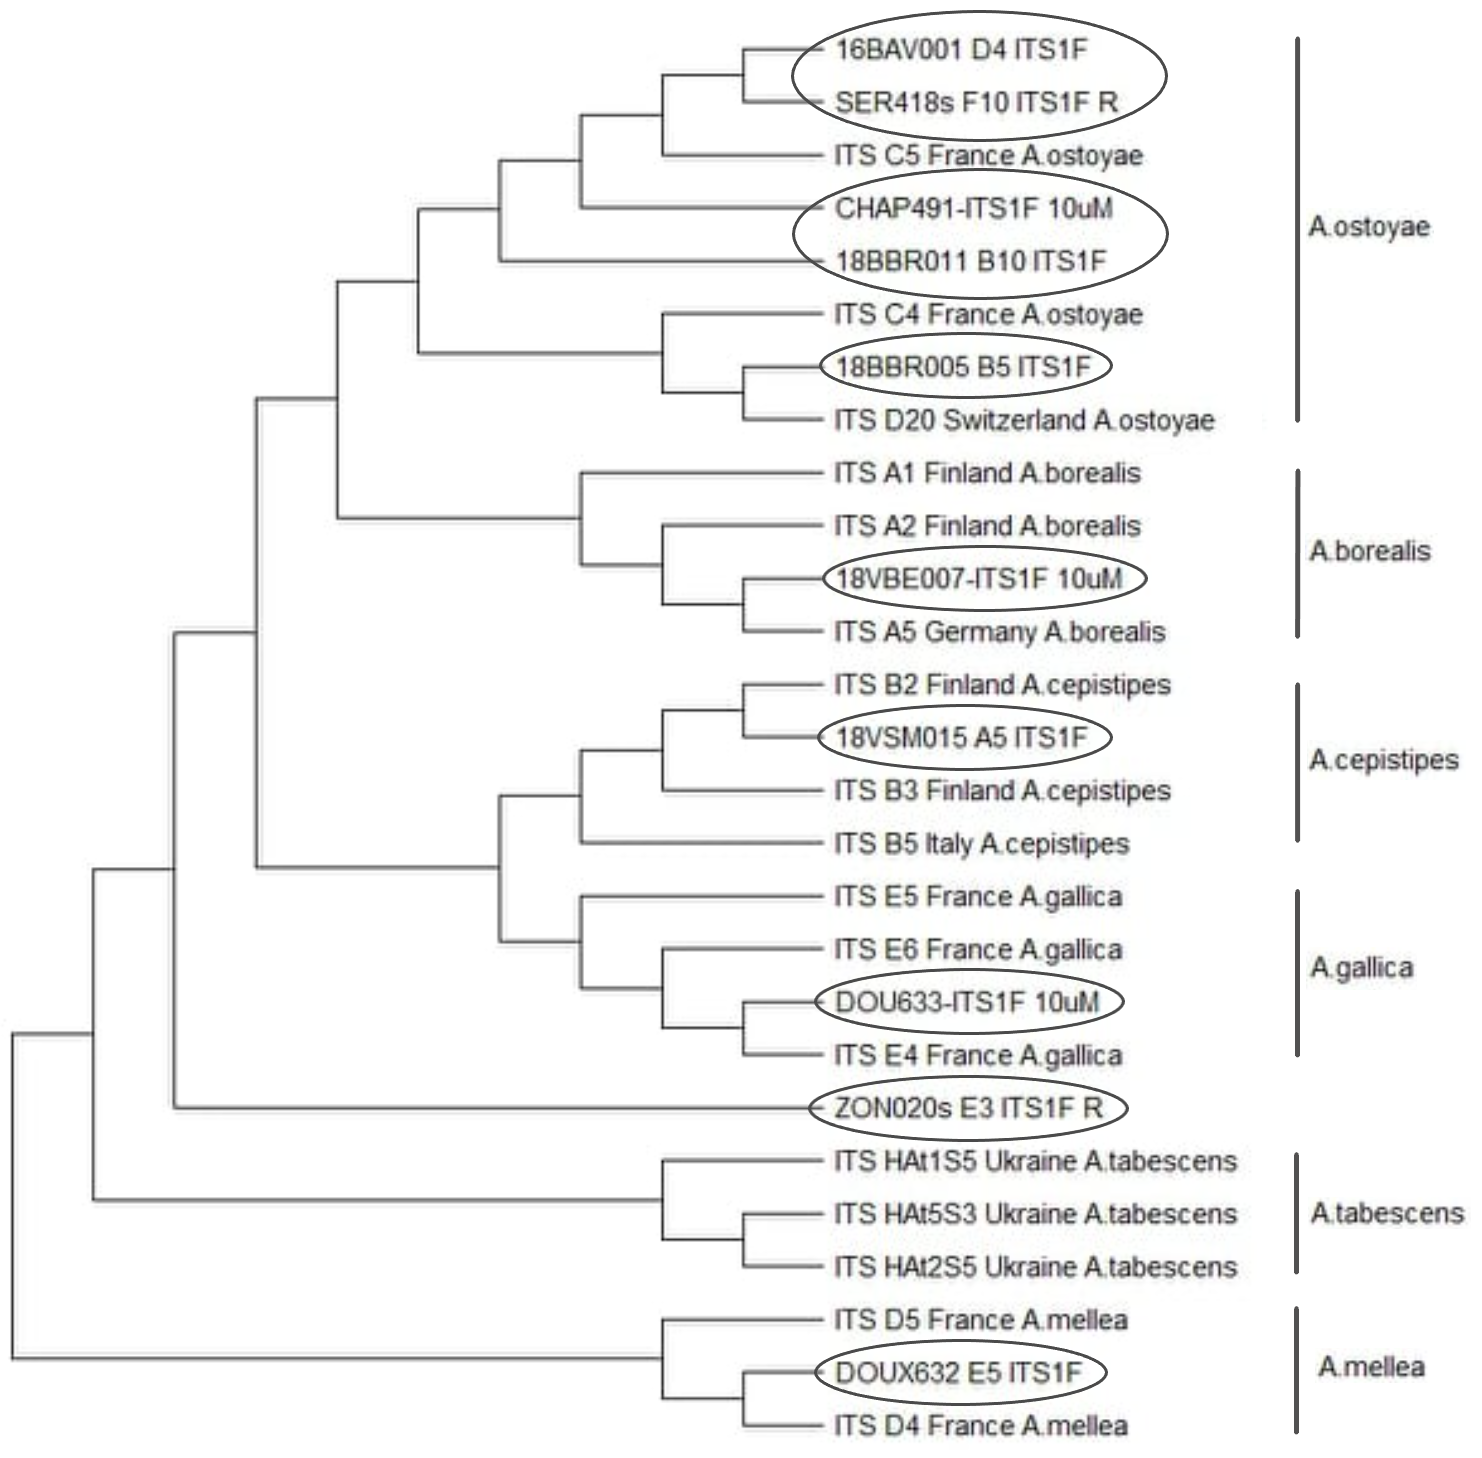
\includegraphics[scale=0.4]{figures/tree_snippet}
\begin{flushright}
\textit{Figure 3 - Arbre phylogénétique des séquences identifiées par rapport aux séquences de référence}
\end{flushright}
\end{figure}

A l'analyse conjointe de ces résultats nous pouvons seulement observer une anomalie concernant l'isolat ZON020s\_E3\_ITS1F\_R. Cet isolat à été identifié comme faisant parti de \textit{A. ostoyae} par le script mais se retrouve en dehors dans l'arbre. Cependant, il ne semble pas se rapprocher d'une autre espèce pour autant, sa position est donc sûrement due à une séquence contenant trop de données manquantes.

\section{Conclusion}
\label{sec:Conclusion}

Cette script présente une méthode simple et rapide de détection de SNPs pour un complexe d'espèces et d'identification d'isolats de ce complexe par leur séquence. Et cela pour l'ITS, barcode des champignons. Comme nous avons pu le voir cette méthode n'est pas dépourvue d'erreurs. Elle nécessite donc aujourd'hui une seconde analyse des résultats par l'utilisateur. Ces erreurs sont principalement issues de la grande proximité des espèces du complexe Armillaire ainsi que le grand polymorphisme de ces espèces. Cela permet un questionnement des espèces fixées actuellement et de leur valeur épistémologique. Les premières recherches à ce sujet avaient menées à l'identification d'une cinquantaine d'espèces d'Armillaires par des critères morphologiques. Des critères biologiques ont permis de réduire ce nombre et les critères phylogénétiques de le fixer à 7 pour les espèces européennes (\textit{A. ectypa} en faisant parti, bien que présent que dans de très peu d'endroits). Récemment certaines espèces d'Armillaire ont vu leur appartenance à ce complexe questionnée et ont été rattachée à un nouveau complexe, Desarmillaria \cite{Park2018}. Et cela peut nous mener à questionner l'illusion de discontinuité que l'on place avec le concept d'espèce. Nous pouvons illustrer cette illusions par le paradoxe sorite \cite{Beth1954}, aussi connu sous le nom de paradoxe du tas :
\begin{itemize}
    \item Un grain de sable ne constitue pas un tas de sable
    \item L'ajout d'un grain de sable ne permet pas de passer d'un non-tas  à un tas
\end{itemize}
Ce paradoxe comporte un biais, contenu intrinsèquement dans sa propre définition. Le concept de tas aurait-il une existence en elle-même ? Pour certains chercheurs, la même question se pose pour le concept d'espèce \cite{Lherminier2005, Hart2011}, qui serait alors plus une commodité de langage plutôt qu'un réel niveau phylogénétique, au même titre que le genre ou la population. Ainsi le continuité que l'on peut définir dans une espèce s'appliquerait à l'ensemble de l'arbre du vivant.

\section{Ressources}

Ce document à été généré par Overleaf, éditeur LaTeX en ligne. Vous pouvez retrouver le code source ici : \url{https://www.overleaf.com/read/cfghtqjhxgts}.

Le script est disponible sur un repository GitHub ici : \url{https://github.com/nobabar/Armillaria}

